\message{ !name(MaximaTut_IISTFOSS.tex)}%-*-EMaxima-*-
\documentclass[12pt,usenames,pdftex]{beamer}

\usetheme{DetlevCM}
\usecolortheme{whale}

\usepackage{verbatim}
% \usepackage{graphics}
\usepackage{lmodern}
\usepackage[lines]{emaxima}
\usepackage{url}

\newcommand{\emx}{\textsl{\sffamily EMaxima}}
\newcommand{\mx}{\textsl{\sffamily Maxima}}
\newcommand{\hyph}{-\hspace{0pt}}
\newdimen\firstcol
\firstcol=.35\textwidth
\newdimen\secondcol
\secondcol=.65\textwidth

\title[Maxima]{A Tutorial Introduction to Maxima}

\author{Nidish Narayanaa B}

\institute[IIST]
{
  Department of Aerospace Engineering\\
  Indian Institute of Space SCience \& Technology, Trivandrum
}

\date[IISTFOSS, 17]{FOSS Group, IIST, 2017}

% \logo{
\includegraphics[width=\linewidth]{Figs/V0}}
\subject{MaximaTut_IISTFOSS}

\AtBeginSection[]{
  \begin{frame}<beamer>{Outline}
    \tableofcontents[currentsection]{}
  \end{frame}
}

\begin{document}

\message{ !name(MaximaTut_IISTFOSS.tex) !offset(-3) }

% \begin{frame}
%   \titlepage{}
% \end{frame}
\maketitle{}
\section{Introduction}

\begin{frame}
  \frametitle{What is Maxima?}
  \begin{quotation}
    (From the website)
    Maxima is a system for the \textbf{manipulation of symbolic and
      numerical expressions}, including differentiation,
      integration, Taylor series, Laplace transforms, ordinary
      differential equations, systems of linear equations,
      polynomials, sets, lists, vectors, matrices and tensors.
  \end{quotation}
\end{frame}

\begin{frame}
  \frametitle{What is Maxima?}
  \begin{itemize}
  \item Powerful Computer Algebra System (CAS) combining symbolic,
    numerical, and graphical capabilities
  \item Cousin of the commercial Macsyma CAS (currently available
    without support)    
  \item Completely Free and Open Source Software, written in LISP
  \item Fully customizable and extensible
  \end{itemize}
\end{frame}

\begin{frame}[<1->]{Interface}
  \frametitle{Interface}
  \begin{columns}
    \begin{column}{0.35\linewidth}
      \begin{description}
      \item<1->[maxima] Native CLI
      \item<2->[xmaxima] History :)
      \item<3->[wxmaxima] Wxwidgets
      \item<4->[imaxima] Emacs!
      \end{description}
    \end{column}
    \begin{column}{0.65\linewidth}
      \begin{center}
        \only<1>{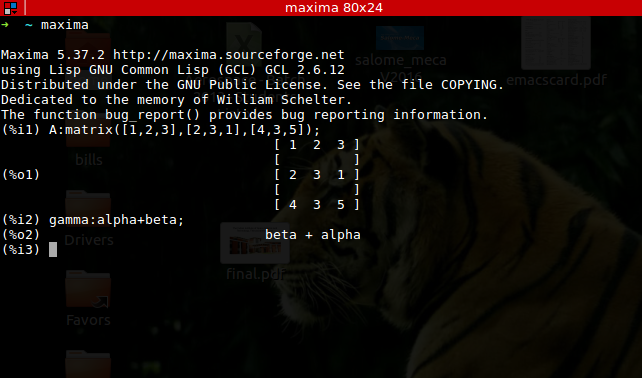
\includegraphics[width=\linewidth]
          {Figs/cli}} 
        \only<2>{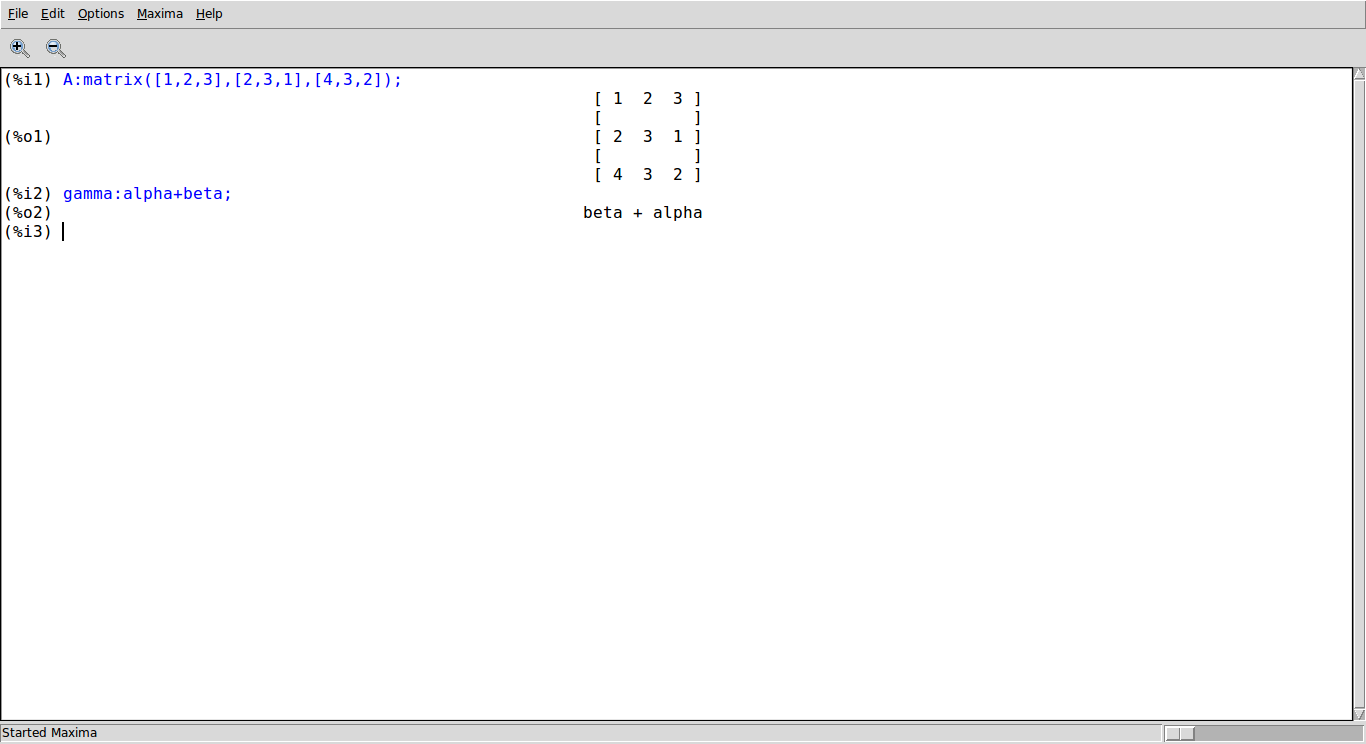
\includegraphics[width=\linewidth]
          {Figs/xmaxima}}
        \only<3,5>{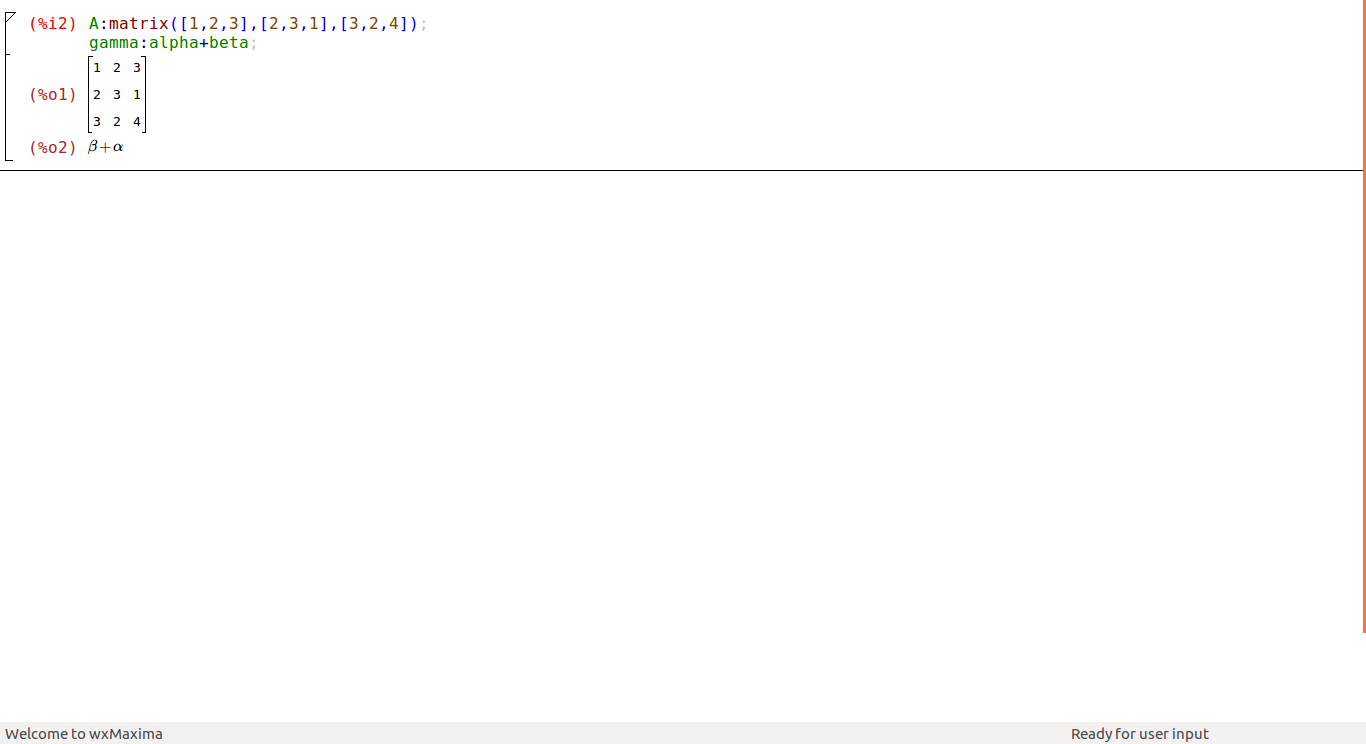
\includegraphics[width=\linewidth]
          {Figs/wxmaxima}}
        \only<4>{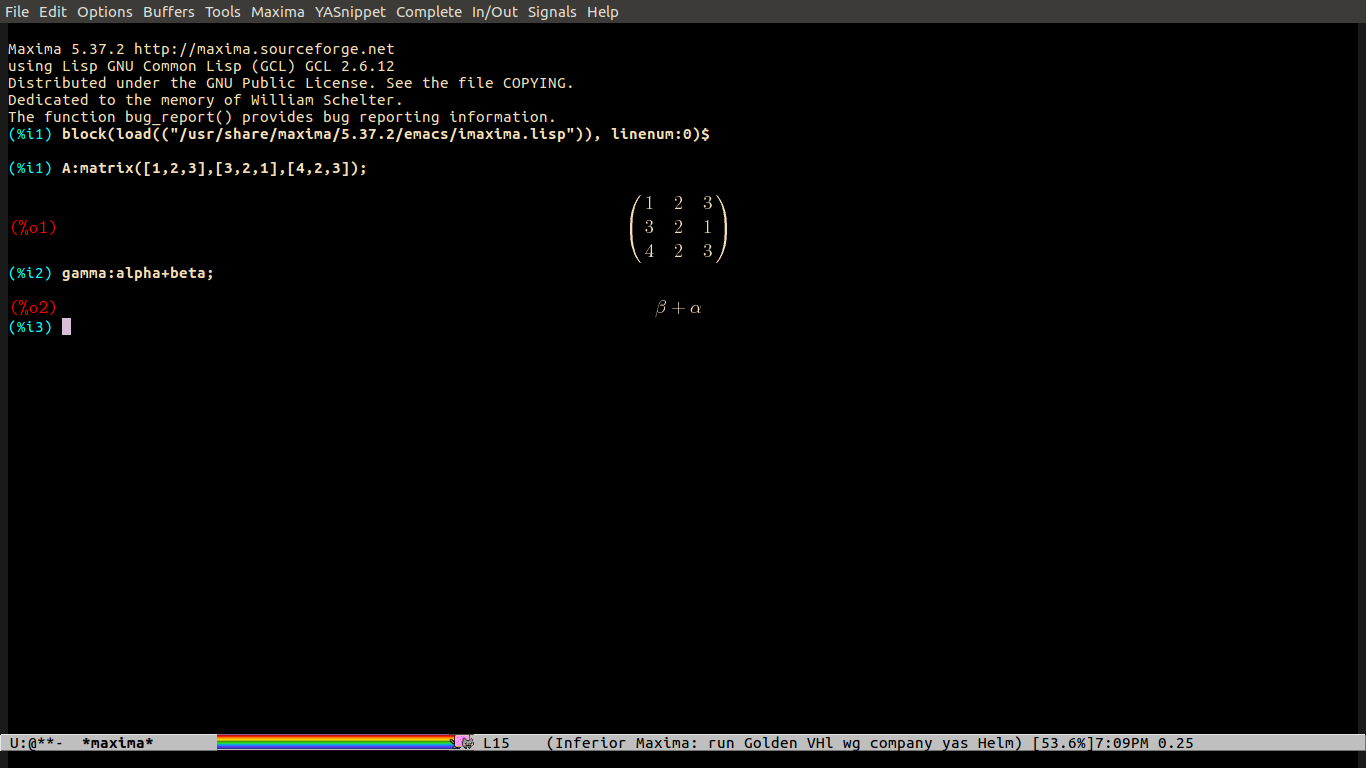
\includegraphics[width=\linewidth]
          {Figs/imaxima}}
      \end{center}
    \end{column}  
  \end{columns}
\end{frame}

\section{Plots and Fits}

\begin{frame}
  \frametitle{Some basics}
  \begin{maxima}
    diff(sin(x^2),x);
    integrate(4*x*cos(x),x,0,x);
\maximaoutput*
\m  2\,x\,\cos x^2 \\
  \end{maxima}
% \begin{maximasession}
% diff(sin(x^2),x);
\maximaoutput*
\i22.  % diff(sin(x^2),x); \\
\p
incorrect syntax: diff is not an infix operator
%Spacediff(
     ^ \\
% \end{maximasession}
\end{frame}


\section{Solving Equations}

\section[ODEs]{Ordinary Differential Equations}

\section[Calculus]{Some Calculus}

\section{Symbolic Math}

\end{document}


%%% Local Variables:
%%% mode: latex
%%% TeX-master: t
%%% End:

\message{ !name(MaximaTut_IISTFOSS.tex) !offset(-140) }
